\section{Related literature and conceptual framework}

\subsection{Flexible prediction and structural pricing objects}

Machine-learning asset pricing has developed along two related lines. The first uses firm characteristics and flexible interactions to predict individual-stock returns \citep{gu2020empirical,avramov2023machine,leippold2022machine}. The second uses characteristics to estimate time-varying exposures, latent factors, or stochastic discount factors (SDFs) \citep{kelly2019characteristics,gu2021autoencoder,chen2024deep,feng2024deep}. Surveys emphasize that these methods can improve prediction and pricing while accommodating a much larger information set than conventional linear specifications \citep{giglio2022factor,bagnara2024review,karolyi2020new}. Recent work also develops formal significance and model-selection procedures for neural or high-dimensional pricing models \citep{fallahgoul2024significance,feng2026stepwise}.

These results establish the value of flexible functional forms, but they do not make the size of a hidden layer or a fitted bottleneck an economic primitive. A predictor can reduce conditional mean-squared error without spanning an SDF that prices a given asset set. A network with many parameters can generate a concentrated representation, while a compact representation can omit a weakly priced direction. We therefore separate predictive complexity, representation dimension, factor dimension, and pricing dimension, and to evaluate each with an object-specific criterion.

Let $Z_t\in\mathbb{R}^{N_t\times p}$ denote the characteristic panel at date $t$, $h_{K,s}(Z_t)$ a fitted representation with nominal output dimension $K$ and training seed $s$, and $F_{K,s,t+1}$ the resulting factor return or SDF innovation. For test-asset excess returns $R_{t+1}\in\mathbb{R}^{J}$, define pricing moments
\begin{equation}
 g_{K,s}=\E[m_{K,s,t+1}R_{t+1}],
\end{equation}
where $m_{K,s,t+1}$ is the scaled SDF associated with the fitted factors. For a positive semidefinite weighting matrix $W$, the population pricing loss is
\begin{equation}
 \Loss_W(K,s)=g_{K,s}'Wg_{K,s}.
 \label{eq:pricing-loss}
\end{equation}
The empirically sufficient dimension is an argmin of an estimate of Eq.~\eqref{eq:pricing-loss}. It is indexed by $W$, the asset vector $R$, the information set used to construct $h$, the fitting sample, and algorithmic randomness. Without additional restrictions it is not an invariant property of the economy.

\subsection{Latent-factor dimension and weak priced directions}

The econometric literature offers consistent procedures for counting pervasive factors from the eigenvalues of large panels \citep{bai2002factors,onatski2010factors,ahn2013eigenvalue}. Asset-pricing applications, however, attach an additional requirement: a direction must matter for pricing, not merely explain covariance. Characteristic-based factor models and supervised latent-factor methods make this distinction operational \citep{kelly2019characteristics,lettau2020factors}. It becomes especially important when risk prices are weak, when the candidate family is nested, or when additional factors are nearly redundant.

Our question is therefore different from estimating the statistical rank of returns. We ask whether the \emph{smallest pricing-sufficient dimension} can be recovered from feasible out-of-sample losses. Cross-validation is well suited to prediction, but selection of a uniquely minimal model requires stronger separation conditions \citep{shao1993cv,yang2007cv,arlot2010cv}. Proposition~\ref{prop:inconsistency} specializes this point to nested pricing models: when larger models share the same population pricing loss and differ only at a higher stochastic order, the raw validation minimum can continue to overselect with positive probability. The simulation section evaluates the size of that problem under controlled truth.

\subsection{Test assets, weighting geometry, and what is identified}

Classical asset-pricing tests make clear that an SDF is assessed through moment restrictions and that the economic distance from a model depends on the return space and its weighting \citep{hansen1991implications,hansen1997assessing,gibbons1989test,shanken1992beta}. Two-pass inference and specification tests further depend on estimated betas, risk prices, and their sampling error \citep{fama1992cross,jagannathan1996conditional,kan2013pricing}. The choice of test assets is consequential: apparently strong fit can arise when the portfolios have a low-dimensional covariance structure or weak exposure to the disputed direction \citep{lewellen2010skeptical}.

These observations imply that a pricing dimension cannot be reported without its measurement geometry. An equal-weighted loss assigns the same coordinate weight to each sample moment. An HJ-type loss rotates and rescales the moment vector using a return second-moment matrix. The factor sets of \citet{fama1993common} and \citet{fama2015five}, characteristic-sorted portfolios, and individual stocks expose different directions. We therefore cross test dimension choices across asset systems and weighting matrices. Disagreement is not treated as a nuisance robustness failure; it is evidence about which parts of the return space identify the claimed dimension.

\subsection{Factor proliferation, model search, and reproducibility}

The factor-zoo literature shows that searching a large menu requires multiple-testing control, shrinkage, and external replication \citep{harvey2016cross,feng2020taming,hou2020replicating}. Many published predictors weaken after discovery \citep{mclean2016destroy}, a smaller subset carries independent information \citep{green2017characteristics}, and regularization can improve pricing when characteristic portfolios contain weak or redundant signals \citep{kozak2020shrinking}. Formal data-snooping procedures provide benchmarks for judging the best rule selected from many candidates \citep{white2000reality,hansen2005spa,romano2005stepwise}. These studies discipline the search over factors or strategies; our paper applies the same logic to the search over dimensions, seeds, losses, data definitions, and historical windows.

Data construction is part of that search space. Characteristic definitions depend on accounting timing, exchange filters, industry mappings, missing-value rules, and cross-sectional transforms. Missing-data treatment can change both the sample and the learned relation \citep{freyberger2025missing}, while interacting anomalies can make apparently separate signals depend on portfolio construction \citep{muller2025interacting}. We therefore treat the legacy 92-characteristic panel and the lineage-audited 86-characteristic panel as two documented measurements of the information set. The resulting sensitivity is economically informative: a dimension that changes when incompletely traceable features are removed may remain predictive, but it is difficult to interpret as a primitive risk count.

\subsection{Representation geometry and functional relevance}

Deep-network representations often occupy a much smaller region than their ambient width suggests. Effective-rank measures summarize spectral concentration \citep{roy2007rank}; nearest-neighbor and likelihood methods estimate local intrinsic dimension \citep{levina2005mle,facco2017twonn}; and layerwise studies document systematic compression in trained networks \citep{ansuini2019intrinsic}. Neural-collapse results provide an important warning that low-dimensional terminal geometry can be created by the training objective itself \citep{papyan2020collapse}. Curvature estimators address a stronger local geometric object \citep{cao2021curvature}. Our tangent-angle diagnostic is a finite-scale comparison, not an implementation of that paper's Weingarten-map estimator. Our numerical-collapse flag is likewise distinct from classification neural collapse.

Representational-similarity methods address a different issue. SVCCA and related canonical-correlation tools compare learned subspaces \citep{raghu2017svcca,morcos2018cca}, while centered kernel alignment (CKA) is invariant to orthogonal transformations and isotropic scaling \citep{kornblith2019similarity}. These tools reveal concentration and drift, but they do not identify which directions price assets. We test one specific form of functional relevance: whether a geometric statistic adds held-out information about a frozen model-level pricing endpoint after conditioning on nominal factor count. This criterion links the measured activations to pricing performance without treating it as the only possible source of economic relevance.

\subsection{Temporal instability, forecast evaluation, and implementation}

Unknown breaks and multiple structural changes can make a full-sample parameter estimate a mixture of distinct regimes \citep{andrews1993instability,bai1998breaks}. Forecast comparisons must then distinguish unconditional average accuracy from conditional performance and account for nested models \citep{diebold1995accuracy,clark2001nested,giacomini2006conditional}. In unstable environments, adaptive combinations can help, but estimation noise and detection delay can erase their theoretical advantage \citep{elliott2004combinations,giacomini2010unstable,smith2021break}. The poor historical record of many equity-premium predictors illustrates why a retrospective fit is not enough \citep{welch2008equity}.

In a nonlinear model, updating changes thousands of parameters at once. The relevant question is not whether two fits differ but whether the change moves forecasts toward subsequently realized returns. For a frozen prediction $f_{it}$, an updated prediction $u_{it}$, and realized return $y_{it}$, define $e_{it}=y_{it}-f_{it}$ and $d_{it}=u_{it}-f_{it}$. The exact difference in squared errors is
\begin{equation}
 (y_{it}-u_{it})^2-(y_{it}-f_{it})^2=d_{it}^2-2e_{it}d_{it}.
 \label{eq:update-decomp}
\end{equation}
Averaging Eq.~\eqref{eq:update-decomp} gives $A-2B$, where $A=\E[d^2]$ is adjustment cost and $B=\E[ed]$ is alignment with the error of the frozen model. Updating helps only when alignment is large enough to exceed half the adjustment cost. This identity turns the vague idea of model drift into an economically interpretable tradeoff.

Even a favorable prediction result need not be investable. Naive rules can outperform estimated optimal portfolios because parameter uncertainty is costly \citep{demiguel2009optimal}, and turnover and trading costs can reverse model rankings \citep{detzel2023costs}. We therefore distinguish a retrospective change in $A$ and $B$, a detection rule that uses only lagged information, and a portfolio comparison after costs and multiplicity correction.

\subsection{Four claims and their evidence}

Table~\ref{tab:propositions} distinguishes four claims. They are an organizing framework, not a theorem that all four are necessary for every valid economic model. In particular, a pricing model need not generate trading alpha to be economically meaningful. The implementation criterion applies when the claim concerns a usable updating policy.

\begin{widetable}[!tbp]
\centering
\caption{Four claims about low-dimensional pricing representations}
\label{tab:propositions}
\footnotesize
\begin{threeparttable}
\begin{tabularx}{\textwidth}{@{}p{0.12\textwidth}p{0.23\textwidth}X@{}}
\toprule
Claim & Empirical object & Evidence relevant to the stated claim \\
\midrule
Geometry & Rank or local dimension of activations & Decline across layers that survives normalization, estimator checks, and a collapse diagnostic. \\
Exact $K$ & Minimal sufficient $K$ & Recovery under known truth or a valid penalty/equivalence rule; stability cannot be inferred from a single validation minimum. \\
Stability & Invariance of the selected economic object & Agreement across test assets, loss geometries, data definitions, seeds, and nonoverlapping periods. \\
Real time & Economic value of reacting to change & A lag-feasible detection rule and a net portfolio gain after inference, turnover, and transaction costs. \\
\bottomrule
\end{tabularx}
\begin{tablenotes}[flushleft]\footnotesize
\item These criteria concern different objects; success on one criterion does not establish the others.
\end{tablenotes}
\end{threeparttable}
\end{widetable}

Figure~\ref{fig:evidence-ladder} tests the geometry--pricing link directly rather than inferring it from visual concentration. For every frozen network, the open marker is its leave-one-seed-out pricing prediction using nominal factor count alone. The arrow ends at the prediction obtained after adding hidden-layer participation rank. If the compressed representation transported reliably into pricing performance, most arrows would move materially toward the 45-degree line. They do not. Representation concentration and incremental pricing information are evaluated separately.

\begin{widefigure}[!tbp]
\centering
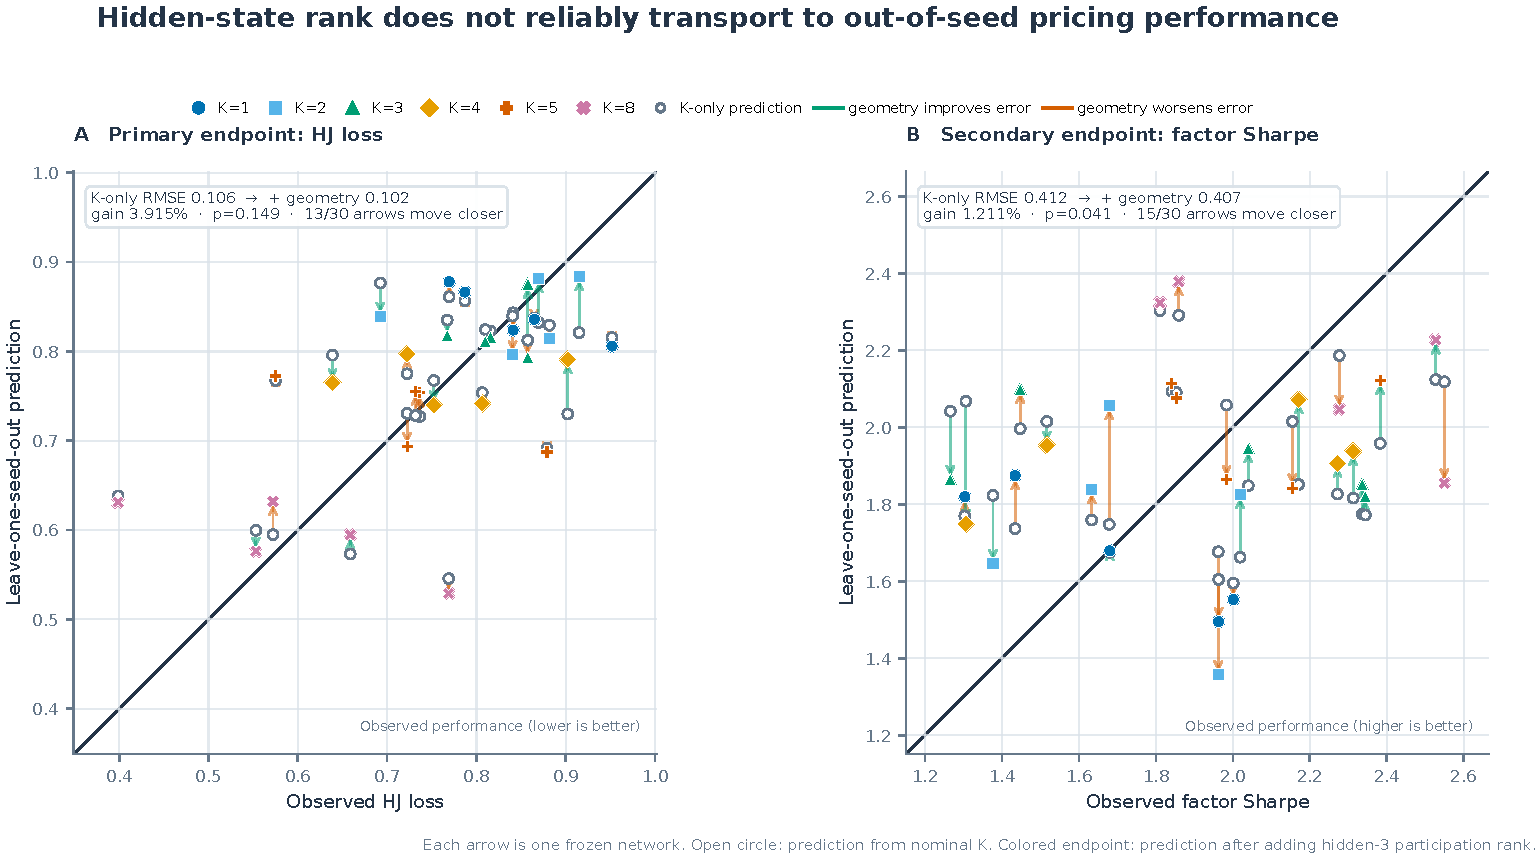
\includegraphics[width=0.98\textwidth]{figures/figure_01_evidence_ladder.pdf}
\caption{Leave-one-seed-out pricing predictions with and without hidden-state geometry. Each arrow is one of 30 frozen networks. Open circles use nominal factor count alone; colored endpoints add hidden-3 raw-centered participation rank, with color and shape identifying nominal $K$. Arrows ending closer to the 45-degree line improve prediction. Geometry reduces HJ-loss RMSE by 3.915\%, below the prespecified 5\% gate ($p=0.149$), and reduces factor-Sharpe RMSE by only 1.211\%. The figure displays the prediction errors behind those aggregate gates rather than rescaled diagnostic ranks.}
\label{fig:evidence-ladder}
\end{widefigure}

\subsection{Why minimum validation loss need not select the minimal dimension}

We give an exact calculation for the known-loading Gaussian design used in Section~4. This is a result about a finite nested family of linear pricing spans, not a consistency theorem for independently trained neural networks.

Let $W$ be fixed and positive definite, and let $P_K$ be the $W$-orthogonal projector onto the span of the first $K$ columns of a full-column-rank loading matrix. The candidate set is finite and contains the smallest correct dimension $K_0$, with $P_{K_0}\mu=\mu$. Independent training and evaluation means satisfy
\begin{equation}
 \bar R_n=\mu+n^{-1/2}U,\qquad
 \bar R_T^{e}=\mu+T^{-1/2}V,
\end{equation}
where $U,V$ are independent $N(0,\Sigma)$ and $\Sigma$ is positive definite. Fit $\widehat\mu_K=P_K\bar R_n$ and evaluate
\begin{equation}
 \widehat\Loss_T(K)=\|\bar R_T^{e}-\widehat\mu_K\|_W^2,
 \qquad \|x\|_W^2=x'Wx.
\end{equation}
For $K>K_0$, put $Q_K=P_K-P_{K_0}$. Orthogonality gives the exact identity
\begin{equation}
 T\{\widehat\Loss_T(K)-\widehat\Loss_T(K_0)\}
 =\frac{T}{n}\|Q_KU\|_W^2
 -2\sqrt{\frac{T}{n}}V'WQ_KU.
 \label{eq:nondegenerate-diff}
\end{equation}

\begin{proposition}[Raw validation selection in the known-loading design]
\label{prop:inconsistency}
Suppose $n/T\to c\in(0,\infty)$ and the candidate set includes at least one $K>K_0$. If every smaller candidate has $\|(I-P_K)\mu\|_W^2>0$, under-selection vanishes but the probability that the unpenalized validation minimizer differs from $K_0$ stays bounded away from zero.
\end{proposition}

Conditional on $U$, the second term in Eq.~\eqref{eq:nondegenerate-diff} is a nondegenerate normal variable whenever $Q_KU\ne0$, an event of probability one. It therefore exceeds the first term with positive probability. An overfitted candidate then beats $K_0$, even as the unscaled loss difference converges to zero. Underfitted candidates instead retain a fixed positive population gap. Supplement~A gives the full argument.

\begin{corollary}[A sufficient penalty rate in this design]
\label{cor:penalty}
For the same finite candidate family, minimizing $\widehat\Loss_T(K)+p_TK$ consistently selects $K_0$ if $p_T\to0$ and $Tp_T\to\infty$.
\end{corollary}

The penalty dominates every $O_p(T^{-1})$ overfit difference while remaining smaller than each fixed underfit gap. With oracle evaluation of the population mean, the cross term in Eq.~\eqref{eq:nondegenerate-diff} is absent and an overfitted candidate cannot improve on $K_0$. Thus the simulation isolates evaluation noise without estimating loadings or the covariance matrix. An estimated weight matrix, different training-to-validation ratio, growing candidate set, or nonlinear fitted family requires a separate analysis. The penalty result is a theoretical benchmark; this paper does not report an empirical comparison of penalty choices.
